\section{Red-Black Tree}

\subsection{Definition and Properties}

\vspace{\parskip}

\begin{definition}[Red-Black Tree] \index{red-black tree}
    A red-black tree is a binary search tree in which every node is either red or black and satisfies the following properties:
    \begin{enumerate}
        \item The root is black
        \item Every leaf node (\textsc{nil} node) is black
        \item If a node is red, then both its children are black
        \item For each node, all paths from the node to descendant leaves (\textsc{nil} nodes) contain the same number of black nodes
    \end{enumerate}
    Alternatively, the properties can be stated without using the \textsc{nil} node.
    \begin{enumerate}
        \item The root is black
        \item A red node has no red children
        \item Every path from the root to a node with at most one child contains the same number of black nodes
    \end{enumerate}
\end{definition}

Figure \ref{fig:rbtree} illustrates the properties of red-black trees.

\begin{figure}[hp]
    \centering
    \includegraphics[width=\linewidth]{rbtree_nil.pdf}
    \includegraphics[width=\linewidth]{rbtree.pdf}
    \caption{Red-black trees. The first tree is represented with the \textsc{nil} sentinel node. The second tree is without the \textsc{nil} node. The two trees are equivalent and both satisfies the red-black tree properties.}
    \label{fig:rbtree}
\end{figure}

\begin{lemma}
    The number of nodes in a red-black tree of height $h$ is at least $2^{\left\lceil (h+1)/2 \right\rceil} - 1$.
\end{lemma}

\begin{proof}

    A red-black tree of height $h$ has a path of length $h$ from the root to a leaf node. This path contains $h+1$ nodes, the first of which is black. Since it does not contain two consecutive red nodes, the path contains at least $b = \left\lceil (h+1)/2 \right\rceil $ black nodes (i.e. at least half of the nodes on that path are black). Hence, every path from the root to a node with at most one child contains at least $b$ black nodes.
    It suffices to prove that there are at least $2^b-1$ black nodes in a red-black tree of height $h$ such that the number of black nodes in the path from the root to a leaf node is $b$. 

    \textsc{Base Case:} If the height of the tree is $0$, then the number of nodes is $1$.

    \textsc{Inductive Step:} Let $h \in \N$ be arbitrary. Assume that for all tree with height $h' < h$, there are $2^{b'}-1$ black nodes where $b'$ is the number of black nodes in the path from the root of that tree to a leaf node. 

    Consider an arbitrary tree $T$  with height $h$ with two subtrees. It follows that there are $b = \left\lceil (h+1)/2 \right\rceil$ black nodes from the root of the tree to a leaf node. If the subtree has a black root, then the path going from the root of the subtree to a leaf contains $b-1$ black nodes. If the root is red, then the path contains $b$ black nodes. Therefore, the number of black nodes in the path from the root of the tree to a leaf node is $b-1$ or $b$. Then, by induction hypothesis, the number black nodes in each subtree is at least $2^{b-1}-1$.

    Since the root of a red-black tree is black, the number of black nodes in $T$ is the number of nodes in the left subtree plus the number of nodes in the right subtree plus the root node.

    $$
    \left( 2^{b-1}-1 \right) + \left( 2^{b-1}-1 \right) + 1 = 2^{b}-1
    $$

    By induction, the number of black nodes in a red-black tree of height $h$ is at least $2^{b}-1 = 2^{\left\lceil (h+1)/2 \right\rceil} - 1$.

\end{proof}

\begin{corollary}
    A red-black tree with $n$ nodes has height $h \leq 2\log_2 (n+1)-1$. 
\end{corollary}

It follows immediately from this corollary that the $\textsc{Search}$ operation will run in $O(\lg n)$ time on a red-black tree.

\section{Insertion and Deletion in Red-Black Tree}

\subsection{Rotation Operations}

It is obvious that $\textsc{Insert}$ and $\textsc{Delete}$ will also run in $O(\lg n)$ time, but the resulting tree may not satisfy the red-black tree properties, meaning that the tree after insertion and deletion of nodes may not be a red-black tree. We can fix this using a technique known as rotation.

\subsection{Insertion}

\begin{codebox}
    \Procname{$\proc{Insert}(T,z)$}
\end{codebox}

We want to first deal with the cases where simple recoloring can fix the problem. We need to determine what color should the newly inserted node be.

If the tree is empty, $z$ should be black. 

If the tree is not empty and the newly inserted node has a black parent, we can make the new node red. This will fix the violation.

If the tree is not empty and the newly inserted node has a red parent, we cannot easily fix the violation by recoloring. If we let that newly inserted node be black, it may lead to a violation of property 3, and if we let the new node be red, it will violate property 2 because it has a red parent.

Suppose that the parent $p$ of the new node is red. Then, $p$ will satisfy the following properties.

\begin{itemize}
    \item $p$ has a black parent $g$ because of property 2;
    \item the parent has no other child other than the newly inserted node. This is because because of property 2, $p$'s children must be black, but then by property 3, the black child will violate property 3.
    \item if $g$ has another child, it would be red
\end{itemize}

\subsubsection{$z$ Is a Leaf}

Case 0: $g$ has only 1 child. In this case, we perform a right rotation around $p$ and recolor.

Case 1: $g$ has 2 children, recolor according to Figure \ref{fig:rbtree_case1}. But this might create a new violation at $g$, so we need to fix that. If $g$ is the root, we can simply change it to black. Otherwise, we need to continue the fix-up procedure at $g$. By doing so, we move the violation up the tree.

\subsubsection{$z$ Is an Internal Node}

Now suppose that $z$ is an internal node.

Case 1: $z$'s two children are black, and $P$ has another black child. $G$ is red. In this case, recolor according to Figure \ref{fig:rbtree_case1}.

Case 2: $G$ is black. Recoloring won't work. We need to do rotation.

$z$ is a left child of a right child or right child of a left child (i.e. a zigzag path from $G \to P \to z$). In this case, do a left rotation at $P$ according to Figure \ref{fig:rbtree_case2}. After this operation, the tree falls into the next case.

$z$ is a left child of a left child or right child of a right child (i.e. a straight path from $G \to P \to z$). In this case, do a right rotation at $G$ according to Figure \ref{fig:rbtree_case3}.

\subsubsection{Case 1}

\begin{figure}[htbp]
    \centering
    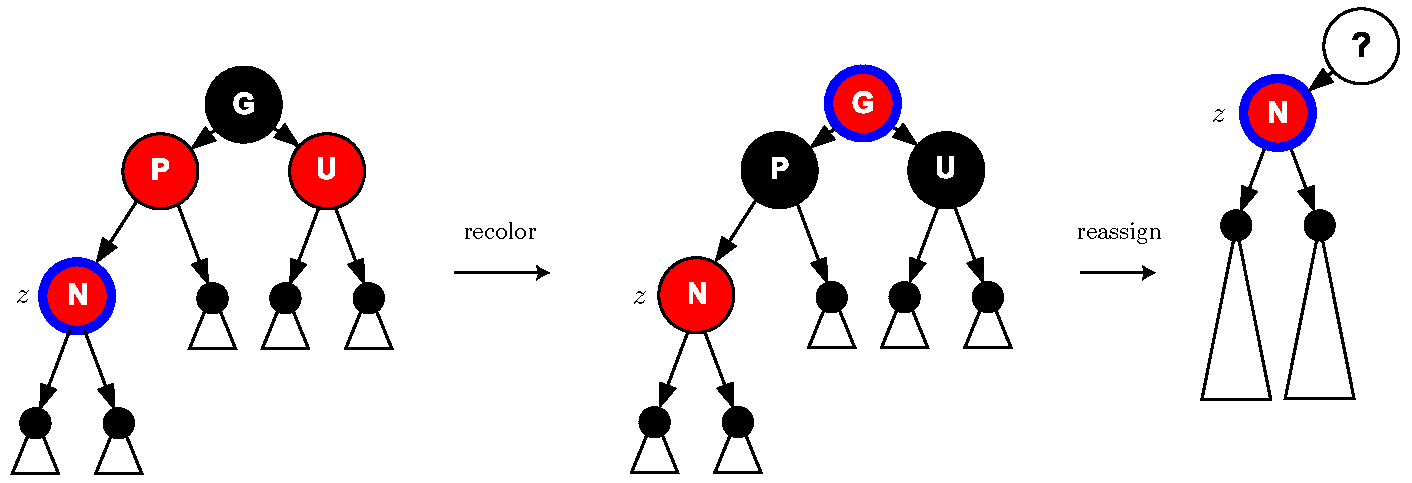
\includegraphics[width=0.9\linewidth]{rbtree_case1.pdf}
    \caption{<caption>}
    \label{fig:rbtree_case1}
\end{figure}

\subsubsection{Case 2}

\begin{figure}[htbp]
    \centering
    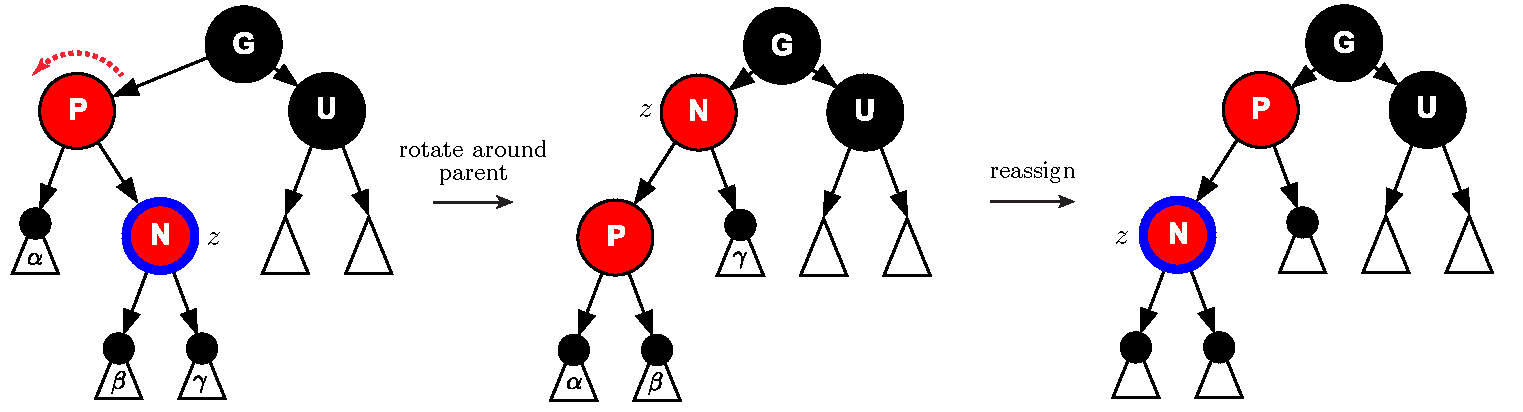
\includegraphics[width=0.9\linewidth]{rbtree_case2.pdf}
    \caption{<caption>}
    \label{fig:rbtree_case2}
\end{figure}

\subsubsection{Case 3}

\begin{figure}[htbp]
    \centering
    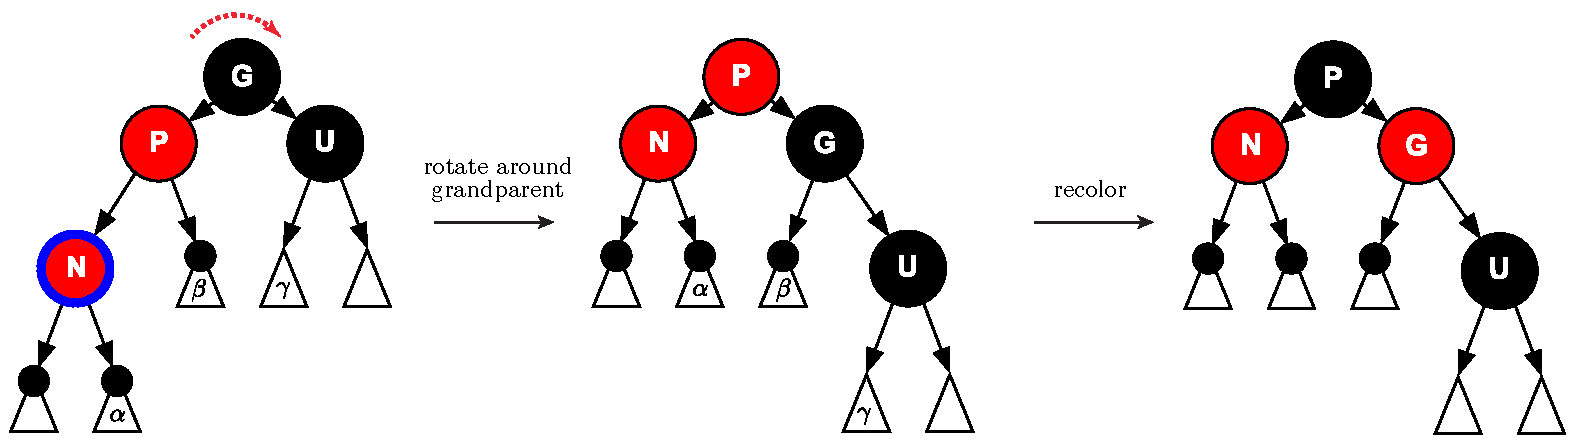
\includegraphics[width=0.9\linewidth]{rbtree_case3.pdf}
    \caption{<caption>}
    \label{fig:rbtree_case3}
\end{figure}

\subsection{Deletion}

Use the BST implementation of $\proc{Delete}(T,x)$. 

When $x$ has two children, we replace $x$ by its successor, which gets the same color as $x$. But then we also need to delete the successor first.

When $x$ has only one child, delete $x$, promote $w$ and make it black.

% x
%  \   to   w
%   w

When $x$ is a red leaf, we can just delete it without recoloring. 

When $x$ is a black leaf, deleting it will cause a violation of property 3, so we need to fix the violation. Let $P$ be the parent of $x$, and let $W$ be the sibling of $x$.

Case 1: $p$ is red.

Case 2: $p$ is black

Case 2(a): $w$ has exactly one child
Case 2(b): $w$ is black and has two children
Case 2(c): $w$ is red and has two children
Case 2(d): $w$ has no children

In Case 2(d), $w$ has to be black. Once $x$ is deleted, we have only $P$ and $W$, which will gives us a black-height of 1 on both sides. This is not fixable, so we make $p$ double-black. And then our goal is to remove the double-black.
